%\documentclass{article}
%\usepackage[a4paper, total={6in, 8in}]{geometry}
\documentclass[reprint,amsmath,amssymb,rmp,onecolumn,notitlepage,11pt]{revtex4-1}
\usepackage[utf8]{inputenc}
%\usepackage{authblk}
%\usepackage{natbib}
\usepackage[normalem]{ulem}
\usepackage{graphicx}
\usepackage{hyperref}
\usepackage{xcolor}
\newcommand{\red}[1]{\textcolor{red!80!black}{#1}}
\newcommand{\blue}[1]{\textcolor{blue!80!black}{#1}}
\newcommand{\green}[1]{\textcolor{green!70!black}{#1}}
\usepackage{mathtools}
\DeclarePairedDelimiter{\evdel}{\langle}{\rangle}

\begin{document}
\title{Linklength distribution in Proteins and our model}
\title{The role of geometry in the chain separation distribution of links in protein contact networks}
%\title{}
%\title{}
%\title{}
\author{Antonia Mey}
\affiliation{EaStCHEM School of Chemistry, University of Edinburgh, Edinburgh, United Kingdom}
\author{Steffen Mühle}
\affiliation{Uni Göttingen, 37077 Göttingen, Germany}
\author{Nora Molkenthin}
\email[Electronic Address: ]{n.molkenthin@gmx.de}
\affiliation{Potsdam Institut für Klimafolgenforschung, Potsdam, Germany}
\affiliation{Chair for Network Dynamics, Institute for Theoretical Physics and Center for Advancing Electronics Dresden (cfaed), Technical University of Dresden, 01069 Dresden}
%\author{Marc Timme}
% \affiliation{Network Dynamics, Max Planck Institute for Dynamics and Self-Organization (MPIDS), 37077 Göttingen, Germany}
% \affiliation{Chair for Network Dynamics, Institute for Theoretical Physics and Center for Advancing Electronics Dresden (cfaed), Technical University of Dresden, 01069 Dresden}

\begin{abstract}
The distribution of chain separations of interacting amino acids in proteins roughly follows a power law. Here we show, analytically and in simulations, that a geometrical stochastic model of folding chains can explain this behaviour. %Separating the data in $\alpha$-dominated, $\beta$-dominated and intrinsically disordered proteins (IDP's) shows characteristic structures in the distribution due to the secondary structure.
\end{abstract}
\maketitle

\section*{Introduction}
Proteins, the molecular machines of every living organism perform vital tasks required for life to persists ranging from transport (e.g. hemoglobin), signal transduction (e.g. rhodopsin), immune responses (e.g. antibodies), and hormonal regulation (e.g. insulin)~\cite{}. All natural proteins are made up of 20 different amino acids which dictate the three dimensional conformations the proteins adopt in order to function~\cite{}. One way of looking at the functional forms of proteins and classifying structure properties of proteins is by looking at protein residue or contact networks~\cite{Vendruscolo2002,DiPaola2013,Estrada2011}. Protein Contact Networks (PCN), 

Since amino acids take up space and are inherently geometrical objects, any plausible network ensemble for describing them, would have to be spatially embedded [5, 10]. Geometrical models for protein folding include models that derive characteristics of the secondary structure from constraints on bond and torsion angles [2, 7] and models focused on the formation mechanisms of the tertiary structure [8]. Based on such considerations, we have constructed a network formation process, in which random connections are added to a chain of unit disks, without causing them to intersect [8]. Here we analyze the link length distribution in those models, where the length of a link is defined as the distance of the two ends along the original chain.
This is then compared to the link length distribution ex- tracted from protein residue networks (PRN) from Pro- tein Data Bank (PDB) data. We find that the frequency of links drops off with their length as
f(l) ∝ l−γ, (1)
both for the model and the PRNs (see Fig. 2), although the PRNs show a dip in the distribution for small lengths. Here f(l) denotes the frequency of links of length l. Interestingly in [https://iopscience.iop.org/article/10.1088/1478-3975/4/4/L01/fulltext/], such a link length distribution (with γ = 1) was imposed on a model (without further explanation), reproducing protein-like average shortest path lengths and clustering coefficient.
\begin{enumerate}
    \item Proteins are very important \cite{a bunch of stuff}
    \item Proteins can be modeled as networks of amino acids and their connections \cite{Vendruscolo2002,DiPaola2013,Estrada2011}.
    \item They postulate/observe that proteins have a sequence separation distribution, that is 1/l in \cite{bartoli2008effect}.
    \item Here we explain this from geometric constraints alone using a model introduced in \cite{Molkenthin2016,molkenthin2020self}
\end{enumerate}
TO DO: Write text
\section*{Model}
\begin{enumerate}
    \item Model in General
    \item Simplified 2D version
\end{enumerate}
TO DO: Write text
\section*{Analytic approximation}
Starting from a closed chain of $N$ unit discs, as introduced for the analytic calculations in \cite{molkenthin2016scaling}. \red{briefly explain that here too.}
Let us start by introducing the auxiliary variable $F(s)$, defined to be the number of possible links with a sequence separation of $s$. Before any links are added all sequence separations are equally likely, as there are $N$ possibilities of making a link of each separation $s$ with $2\leq s < N/2$.

As we add more links, not only are links taken out of this pool, because they have already been realized, each existing link can also geometrically prohibit other connections.
Let us call the pools of available links after $i$ links have been added $F_i(s)$.
\begin{figure}
    \centering
    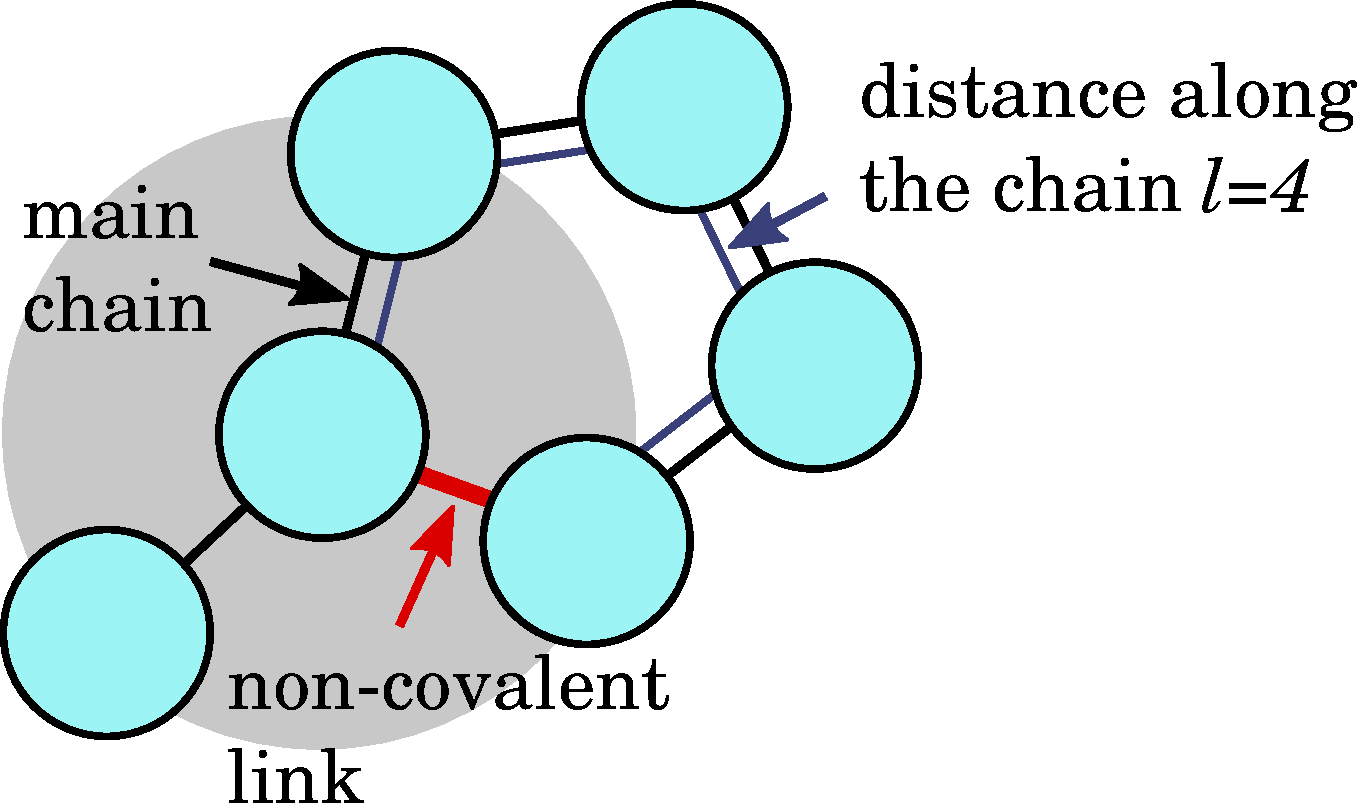
\includegraphics[width=\columnwidth]{prn_vis.pdf}
    \caption{Caption}
    \label{fig:fig_prn_vis}
\end{figure}

-------------- Add Figure explaining which links are geometrically excluded --------------

The expected distribution of possible links after one step is given by the average over available link pools taken over all possible lengths of the initial link
\begin{equation}
    F_1(s)= \frac{1}{N/2-2} \sum_{s_1=2}^{N/2} { \begin{cases}
    N-2(s-1) \text{ , for } s<s_1\\
    N-2(s_1 -1)\text{ , for } s\geq s_1
    \end{cases}}.
\end{equation}

In subsequent steps we get the same reduction but starting from the pool of the step before rather than the full $N$ links for each length, leading to an additional probability factor \red{explain this in more detail, I already forgot exactly why that is...}
\begin{equation}
    P_k(s)=\frac{F_k(s)}{C_k},
    \label{eq.Pk}
\end{equation}
with $C_k=\sum_{s=2}^{N/2}F^k(s)$, for each segment separation $s$ to occur and thus
\begin{equation}
    F_k(s)= \frac{1}{N/2-2} \sum_{s_k=2}^{N/2} {\begin{cases}
     F_{k-1}(s)-2(s-1) P_k(s) \text{ , for } s<s_k\\
     F_{k-1}(s)-2(s_k -1)P_k(s)\text{ , for } s\geq s_k
    \end{cases}}.
\end{equation}
This can be simplified to
\begin{align}
   F_k(s)&= \frac{1}{\frac{N}{2}-2} \frac{F_{k-1}(s)}{C_{k-1}}\left( \sum_{s_k=2}^{N/2}C_{k-1} - \sum_{s_k=2}^{s} 2(s_k-1) - \sum_{s_k=s+1}^{N/2} 2(s -1) \right) \nonumber \\
   &= \frac{1}{\frac{N}{2}-2}\frac{F_{k-1}(s)}{C_{k-1}}\left(\left(\frac{N}{2}-2\right)C_{k-1} -(s^2-s)-2\left(\frac{N}{2}-(s+1)\right)(s-1)\right)  \nonumber \\
   &= F_{k-1}(s)\left(1-\frac{-s^2 +(N-1)s-(N+1)}{(\frac{N}{2}-2)C_{k-1}} \right)\nonumber \\
   &=F_{k-1}(s)\left(1-\frac{f(s)}{(\frac{N}{2}-2)C_{k-1}} \right)
   \label{eq.Fk_rec}
\end{align}
Where we defined $f(s)=-s^2 +(N-1)s-(N+1) \approx N s - s^2 - N$ for notational brevity.

We can now use the recursive expression Eq.~\ref{eq.Fk_rec} to write down a closed expression for $F_k(s)$

\begin{equation}
    F_k(s)=N\prod_{i}^k\left(1-\frac{f(s)}{(\frac{N}{2}-2)C_{i-1}} \right)
\end{equation}

The probability distribution of the realized sequence separations of all added links is then given by the average over the available pools at each link addition step, leading to
\begin{align}
    P(s)&=\frac{1}{N-3}\sum_{k=0}^{N-3} P_k(s) \nonumber \\
    &= \frac{N}{N-3}\sum_{k=0}^{N-3} \frac{1}{C_k}\prod_{i}^k\left(1-\frac{f(s)}{(\frac{N}{2}-2)C_{i-1}} \right),
\end{align}
which makes use of Eq.~\ref{eq.Pk}. The only unknown in this expression is $C_k$, which we can not compute exactly. However, since $C_k$ monotonically decreases with $k$, $N>C_k>C_{N-2}$ always holds and we can obtain an upper and lower bound by replacing all $C_k$ in the expression with either $N$ (underestimates all probabilities) or $C_{N-2}$ (overestimates all probabilities). Each time we get an expression of the form 
\begin{align}
     P(s)&\approx\frac{N}{N-3}\sum_{k=0}^{N-3} \frac{1}{C_k}\prod_{i}^k\left(1-\frac{f(s)}{(\frac{N}{2}-2)C} \right)\nonumber \\
     &=\frac{N}{N-3} \sum_{k=0}^{N-3}\frac{1}{C_k}\left(1-\frac{f(s)}{(\frac{N}{2}-2)C} \right)^k \nonumber \\
     &\approx \frac{A}{f(s)}
\end{align}
for $1<s<\frac{N}{2}$,
where $A$ is an unknown constant, containing an approximation of the various normalization constants $C_i$, as well as the direct effects of the chain length. 
Since for long chains, $f(s)$ is largely dominated by the linear term, the distribution is well approximated by a power law with an exponent of $-1$. We have made use of the geometric series to approximately find a closed solution. 

In the last step of this approximation, we take the $C_k$ to all be approximately equal in order to apply the geometric series. However, in reality we know $1/C_k$ to increase with $k$, giving large $k$ summands relatively more weight than in a geometric series. This would lead to a correction in the exponent.

\begin{equation}
    P_{corrected}(s)\approx A f(s)^{-1+\alpha},
\end{equation}
where $0<\alpha<1$ \red{why cant $\alpha$ be >1?}.


\section*{Data and simulations}
 For large values of the chain length $N$ we thus find an approximate power law probability distribution for the sequence separation with an exponent of -1 \red{include note of correction}. Here we use simulations, as introduced in \cite{molkenthin2020self} and networks extracted from measured protein data from the PDB \cite{PDB} to compare this behaviour in realistic 3D settings and show that the basic principle persists, indicating that the sequence distance separation distribution is largely determined by simple geometric constraints.
 
The complex interaction pattern between the amino acids in a protein can be very naturally expressed as a network, in which each amino acid is represented by a node and spatial proximity is encoded as a link. Whenever two central $C_\alpha$ atoms are closer together than a threshold $d_c$, they are connected. These connections are encoded in the adjacency matrix, which is the binary matrix
\begin{equation}
  A^{\textsf{PDB}}_{ij}=
  \begin{cases}
   0, & \text{ if } d_{i,j}>d_c \text{ or } i=j\\
      1, & \text{ if } d_{i,j}\leq d_c .
      \end{cases}
    \label{eq:aij}
\end{equation}
  
\begin{figure}[h]
        \centering
	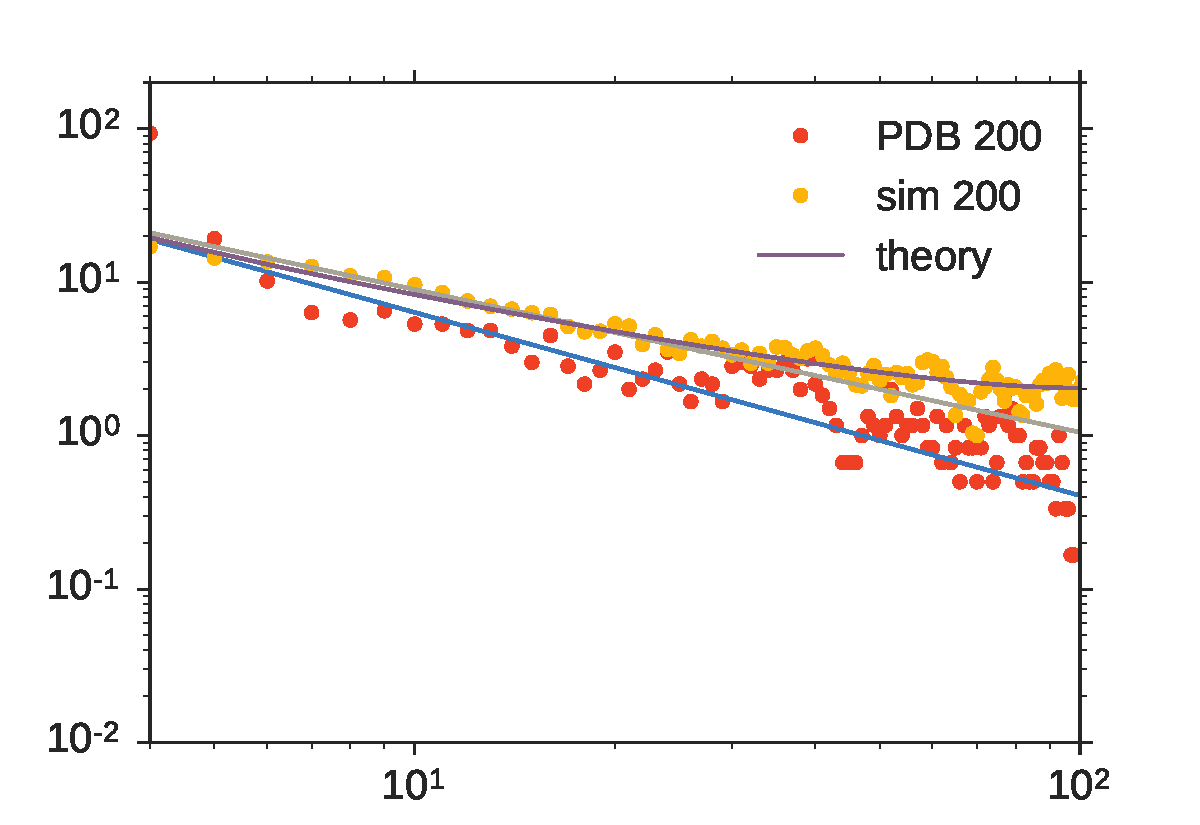
\includegraphics[width=0.45\textwidth]{figures/idp_200.pdf}
	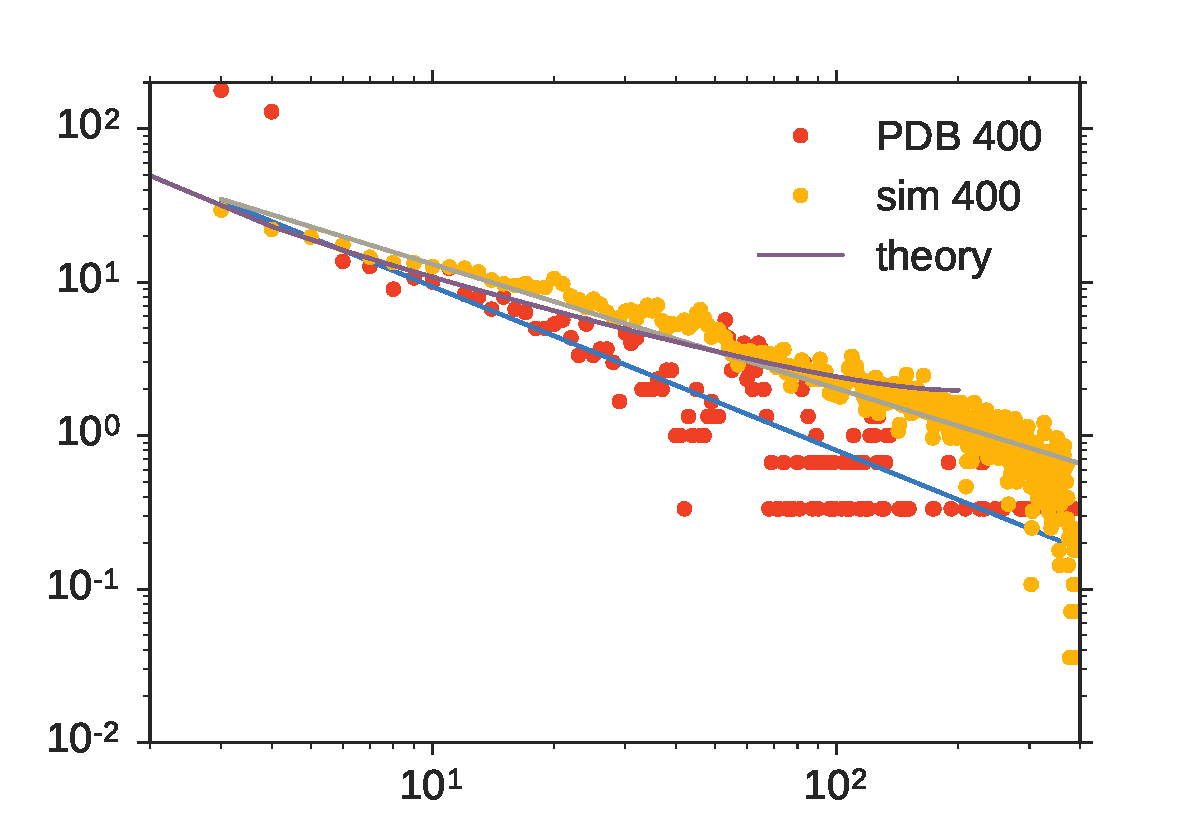
\includegraphics[width=0.45\textwidth]{figures/idp_400.pdf}
        \caption{Sequence distance distributions for real and simulated folds for a) Chain lengths around 200 b) chain lengths around 400. The theoretical curve for 2D rings works okay for 3D open chains (because the rings are closed sequence separations of more than N/2 are a bit meaningless and thus not accounted for) The parameters used in this are $A=80$ and $\alpha=0.2$ in a) and $0.3$ in b). I thought in b) it makes sense for $\alpha$ to be larger as there are even larger exponents $k$ coming into relevance. I'm not sure we want to use that whole $\alpha$ argument too much though as it's a but ad-hoc and would be nicer to just fit $A$ and be done with it, but then it may look a bit more off.
        }
        \label{fig:time_scaling}
\end{figure}
\section*{Conclusion}
\begin{enumerate}
    \item We can now explain the sequence separation from geometry and even do it analytically.
    \item Maybe something about helixes and sheets and the dip.
\end{enumerate}
TO DO: Leave until the rest is done.
\section*{Declarations}
\subsection{Availability of data and materials}
All data generated or analysed during this study are included in this published article [and its supplementary information files].
\subsection{Competing interests}
The authors declare no competing interests.
\subsection{Funding}
This research was supported by ...
\subsection{Authors' contributions}

\subsection{Acknowledgements}
We thank ... for fruitful discussions.

\bibliographystyle{unsrt}
\bibliography{proteins}

\appendix
\section{Supplemental Material Collection}
\section{Random ideas}
\begin{itemize}
    \item Why is the beginning different for simulations?
    \item Does the dip disappear for IDPs
    \item Can we use all NMR structures for IDPs
    \item Would it help using more simulated structures than just the Crystal structure. 
\end{itemize}
TODO: @Toni: Collect data and plotting scripts in github
TODO: @Toni: Connect overleaf to github \green{(check)}


\end{document}